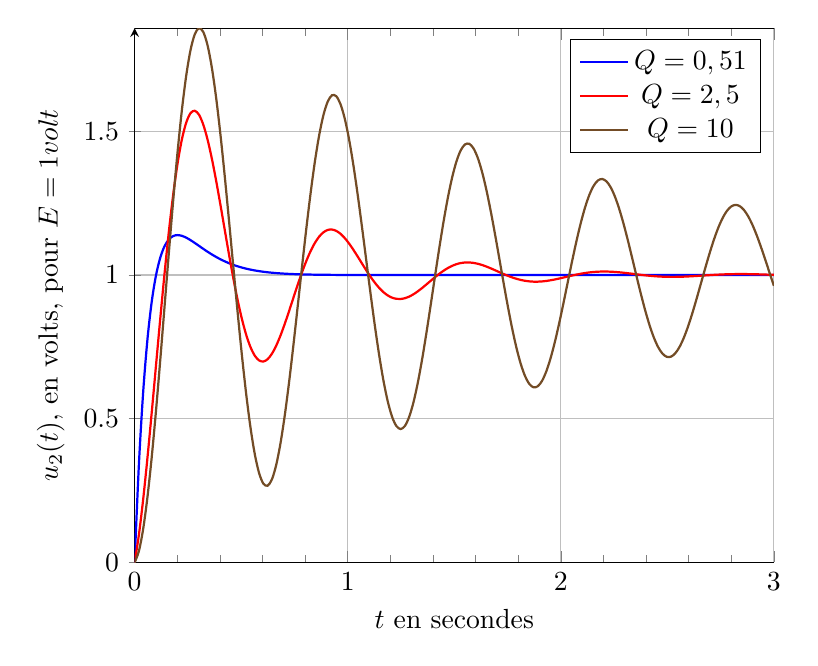
\begin{tikzpicture}[declare function={ 
											omega=10;
											om(\q)=omega*sqrt(1-1/(4*\q*\q));
											tau(\q)=(2*\q)/omega;
											e0=1;
											u(\t,\q)=e0*  exp(-\t/tau(\q)) *(  sin(om(\q)*\t r)/(tau(\q)*om(\q)) -  cos(om(\q)*\t r)) + e0;
											}]

\begin{axis}[width=.8\columnwidth,
                        xmin=0,
                        xmax=3,
                        axis y line=left,
                        ylabel= {$u_2(t)$, en volts, pour $E=\qty{1}{volt}$},
                        xlabel={ $t$ en secondes},
                       grid = major,
	                   xtick={0,1,..., 3},
                       minor x tick num = 4,
                       ]  

\foreach \q in  {0.51,2.5,10} {        
\addplot+[thick, mark=none, samples=150, domain=0:3, smooth] {u(x,\q)};
}
\legend{$Q=\num{0,51}$, $Q=\num{2,5}$, $Q=\num{10}$}
\end{axis}
\end{tikzpicture}